Soit $I$ un intervalle réel tel que $\mathring{I} \neq \emptyset$.

$\K = \R$ ou $\C$, et $E$ est un $\K$-espace vectoriel normé
 de dimension finie.


\section{Dérivation }
\subsection{Dérivée en un point}

\begin{definition}{dérivable en un point}{}
    Soit $a \in I$ et $f: I \to E$. On dit que $f$ est dérivable en $a$ ssi 
    \[\fonction{\Delta_a}{I \setminus \{a\}}{E}{t}{\frac{f(t) - f(a)}{t-a}}\]
    a une limite $\ell \in E$ en $a$. Cette limite est appelée dérivée (ou vecteur dérivé)
    de $f$ en $a$ et se note $f'(a)$.

    On a alors : $\displaystyle \frac{f(a + h ) - f(a)}{h} \xrightarrow[h \to 0]{N} f'(a)$.
\end{definition}

\begin{proposition}{caractérisation de la dérivabilité}{}
    Soit $a \in I$ et $f: I \to E$. Alors $f$ est dérivable en $a$ ssi il existe $V \in E$
    et $\varepsilon : I \to E$, avec $\varepsilon(t) \xrightarrow[t \to a]{} 0$ telle que
    \[f(t) = f(a) + (t-a)V + (t-a)\varepsilon(t)\]

    appelée développement limité de $f$ en $a$ à l'ordre 1, et alors $V = f'(a)$.
\end{proposition}

\begin{proof}
    Si $f$ est dérivable en $a$, posons $V = f'(a)$ et $\varepsilon(t) = \frac{f(t) - f(a)}{t - a }$ si 
    $t \neq a$ et $\varepsilon(a) = 0$. 

    Alors $\varepsilon$ vérifie l'égalité et $\varepsilon$ continue en $a$ car 
    $\displaystyle \frac{f(t) - f(a)}{t-a} \xrightarrow[t \to a]{} f'(a)$, c'est à dire 
    $\varepsilon(t) \xrightarrow[t \to a]{} 0$.

    \uindent{Réciproquement }

    \svspace Si $\varepsilon$ et $V$ existent, $\displaystyle \frac{f(t) - f(a)}{t-a} = V + \varepsilon(t) \limit t a V$
    Donc $f$ dérivable en $a$ et 
    
    $f'(a) = V$.
\end{proof}


\begin{corollaire}{dérivabilité implique continuité}{}
    Si $f$ est dérivable en $a$, alors $f$ est continue en $a$.
\end{corollaire}

\begin{proof}
    En ce cas $f(t) = f(a) + (t-a)f'(a) + (t-a)\varepsilon(t) \xrightarrow[t \to a]{} f(a)$.
\end{proof}


\begin{definition}{interprétation cinématique}{}
    Soit $f : I \to E$ courbe paramétrée. 
    
    $t$ instant et $f(t)$ posittion d'un point matériel à l'instant 
    $t$ $f'(a)$ vecteur vitesse à l'instant $a$. 

    Si $f'(a) \neq 0$, $T = \{ f(a) + hf'(a), \, h \in \R\}$ tangeante à la courbe à l'instant 
    $a$. 

    $C = \{ f(t), \, t \in I\}$ support de la courbe paramétrée par $f$. 
\end{definition}

\begin{proposition}{lien avec une base }{}
    Soit $B = (e_1, \ldots, e_n)$ une base de $E$, et soit 
    $\displaystyle \fonction{f}{I}{E}{t}{\sum_{i=1}^n f_i(t)e_i}$, où $f_i : I \to \R$.

    Soit $a \in I$. $f$ est dérivable en $a$ ssi $\forall i \in \ninter{1}{n}$, $f_i$
    est dérivable en $a$, et alors 
    $$f'(a) = \sum_{i=1}^n f_i'(a)e_i$$
\end{proposition}

\begin{proof}
    $\Delta_a(t) = \displaystyle \frac{f(t) - f(a)}{t-a} = \sum_{i=1}^n \frac{f_i(t) - f_i(a)}{t-a}e_i$ a 
    une limite quand $t \to a $ ssi toutes ses coordonnées ont une limite.
\end{proof}

\begin{exemple}
    $\fonction f \R {\R^3} t {(\cos t, \sin t, t)}$ représente une hélice.
\end{exemple}

\begin{definition}{dérivabilité à droite et à gauche}{}
    Soit $f : I \to E$ et $a \in \mathring I$. 

    \avspace On définit $\fonction{f_g}{I \cap ]-\infty, a]}{E}{t}{f(t)}$ et 

    \avspace $\fonction{f_d}{I \cap [a, +\infty[}{E}{t}{f(t)}$

    Comme $a \in \mathring I$, $I \cap ]-\infty, a]$ et $I \cap [a, +\infty[$ 
    sont d'intérieur non vide.

    On dit que $f$ est dérivable à gauche (resp. à droite) en $a$ ssi $f_g$ 
    (resp. $f_d$) est dérivable en $a$.

    On définit alors le vecteur dérivé à gauche (resp. à droite) de $f$ en $a$ par 
    $\displaystyle f'_g(a) = \lim_{t \to a} \frac{f_g(t) - f_g(a)}{t-a} = \lim_{t \to a^-} \frac{f(t) - f(a)}{t-a}$
    (resp. à droite par $\displaystyle f'_d(a) = \lim_{t \to a^+} \frac{f(t) - f(a)}{t-a}$).                                                    
\end{definition}

\begin{proposition}{dérivabilité en un point avec dérivées à gauche et à droite}{}
    $f$ est dérivable en $a$ ssi elle est dérivable à gauche et à droite en $a$ et
    
    $f'_g(a) = f'_d(a)$. 
\end{proposition}

\begin{proof}
    Coordonnée par coordonnée.
\end{proof}

\begin{definition}{point anguleux, LHP}{}
    Soit $f : I \to E$, et $a \in \mathring{I }$. 
    On suppose que $f$ est dérivable à gauche et à droite en $a$ et que 
    $f'_g(a) \neq f'_d(a)$.

    On dit alors que la courbe paramétrée par $f$ possède en $a$ un point anguleux.
\end{definition}

\subsection{Dérivabilité sur un intervalle}

\begin{definition}{dérivable sur un intervalle}{}
    Soit $f : I \to E$. On dit que $f$ est dérivable sur $I$ ssi elle l'est en tout $a \in I$. 

    On définit alors sa dérivée $\fonction{f'}{I}{E}{t}{f'(t)}$. 

    L'ensemble des fonctions dérivables de $I$ dans $E$ est noté $\mathscr D(I, E)$.
\end{definition}

\begin{definition}{fonction de classe $\mathscr C^1$}{}
    On dit que $f : I \to E$ est de classe $\mathscr C^1$ sur $I$ ssi 
    elle y est dérivable et si $f'$ est continue. 

    L'ensemble de ces fonctions est noté $\mathscr C^1(I, E)$.
\end{definition}

\begin{proposition}{Dérivabilité et classe $\mathscr C^1$ avec une base }{}
    Soit $B = (e_1, \ldots, e_n)$ une base de $E$, et soit
    $\displaystyle \fonction{f}{I}{E}{t}{\sum_{i=1}^n f_i(t)e_i}$, où $f_i : I \to \K$.

    Alors $f$ est dérivable (resp. de classe $\mathscr C^1$) sur $I$ ssi
    $\forall i \in \ninter{1}{n}$, $f_i$ est dérivable (resp. de classe $\mathscr C^1$).
\end{proposition}

\begin{exemple}
    $\fonction{f}{\R}{\R^2}{t}{(x(t), y(t))}$ avec $x(t) = 2 \cos(t)$ et $y(t) = \sin(t)$.

    Alors $f$ est $\mathscr C^1$ sur $\R$ car $x$ et $y$ le sont.
\end{exemple}

\begin{proposition}{Structure fonctions dérivables et $\mathscr C^1$}{}
    $\mathscr D(I, E)$ et $\mathscr C^1(I, E)$ sont des $\K$-espaces vectoriels et 

    $\fonction{}{\mathscr C^1(I, E)}{\mathscr C(I, E)}{f}{f'}$ est linéaire. 
\end{proposition}

\subsection{Composition }

\begin{proposition}{Composition à droite}{}
    Soit $f \in \mathscr C^1(I, E)$ et $\varphi \in \mathscr C^1(J, I)$, où $J$ est un intervalle de $\R$
    tel que $\mathring{J } \neq \emptyset$. 

    Considérons $\fonction{g = f \circ \varphi}{J}{E}{u}{f(\varphi(u))}$.

    Alors $g \in \mathscr C^1(J, E)$ et $g' = \varphi' f' \circ \varphi$
    
\end{proposition}

\begin{remarque}
    (Hors programme)

    La composition par $\varphi$ s'appelle un changement de paramétrage.

    Si $\varphi$ est bijective et si $\varphi^{-1} \in \mathscr C^1(I, J)$, c'est à dire si 
    $\varphi '$ ne s'annule pas (on dit alors que $\varphi$ est un $\mathscr C^1$-difféomorphisme). 

    On dit que $\varphi$ est un changement de paramétrage admissible.
\end{remarque}

\idee{Coordonnée par coordonnée.}

\begin{proof}
    Soit $B = (e_1, \ldots, e_n)$ une base de $E$. 

    Notons $\displaystyle \forall t \in I, \, f(t) = \sum_{i=1}^n f_i(t)e_i$. 

    Alors $\displaystyle \forall u \in J, \, g(u ) = \sum_{i=1}^n f_i(\varphi(u))e_i$. 

    Donc $g \in \mathscr C^1(J, E)$ et $\displaystyle g'(u) = \sum_{i=1}^n \varphi'(u)f_i'(\varphi(u))e_i = \varphi'(u)f'(\varphi(u))$.
\end{proof}

\begin{theoreme}{composition par une application linéaire}{}
    Soit $(F, N)$ un espace vectoriel normé de dimension finie, et $f$ dérivable en $a$
    (resp. sur $I$, resp. de classe $\mathscr C^1$ sur $I$) et $u \in \mathscr{L }(E, F)$.

    Alors $u \circ f$ est dérivable en $a$ (resp. sur $I$, resp. de classe $\mathscr C^1$ sur $I$) et
    
    $(u \circ f)'(a) = u \circ f'(a) $ (resp. $(u \circ f)' = u \circ f'$).

\end{theoreme}

\idee{Passer par le DL de $f$, et composer par $u$.}

\begin{proof}
    \uline{En $a$ :}

    Par hypothèse, pour $t \in I$, $f(t) = f(a) + (t-a)f'(a) + (t-a)\varepsilon(t)$

    En composant par $u$, on obtient $u(f(t)) = u(f(a)) + (t-a)u(f'(a)) + (t-a)u(\varepsilon(t))$.

    Et on a bien $u(\varepsilon(t)) \xrightarrow[t \to a]{} 0$, donc $u \circ f$ dérivable en $a$ et $(u \circ f)'(a) = u(f'(a))$.

    Or ceci est vrai en tout point de $I$, donc $(u \circ f)' = u \circ f'$.

    Si $f \in \mathscr C^1(I, E)$, $u$ étant linéaire entre espaces de dimension finie, elle est continue donc $(u \circ f)'$ 
    est continue. 
\end{proof}

\begin{exemple}
    Résolvons le système 
    \[(S) = \begin{cases}
        x'(t) = 2x(t) + y(t) \\
        y'(t) = 4x(t) - y(t)
    \end{cases}\]

    Posons $X(t) = \begin{pmatrix} x(t) \\ y(t) \end{pmatrix}$ et $x, y$ sont $\mathscr C^1$ 
    de $\R$ dans $\R$. De même, $X$ est $\mathscr C^1$ de $\R$ dans $\R^2$. Donc : 

    $$(S) \Leftrightarrow \forall t \in \R, \, X'(t) = \begin{pmatrix} 2 & 1 \\ 4 & -1 \end{pmatrix} X(t)$$

    Posons $P = \begin{pmatrix} 1 & 1 \\ 1 & -4 \end{pmatrix}$, $P$ est inversible car $\det(P) = -5 \neq 0$.

    Posons $\forall t, \, Y(t) = P^{-1}X(t)$. Comme $\fonction u {\R^2}{\R^2}{M}{P^{-1}M}$ est linéaire, 
    $Y$ est $\mathscr C^1$ et $Y'(t) = P^{-1}X'(t)$ car $Y = u \circ X$ donc $Y' = u \circ X'$.

    Donc $(S) \Leftrightarrow \forall t \in \R, \, Y'(t) = P^{-1} \begin{pmatrix} 2 & 1 \\ 4 & -1 \end{pmatrix} P y(t)$

    Posons $Y(t) = \begin{pmatrix} \varphi(t) \\ \psi(t) \end{pmatrix}$ où 
    $\varphi, \psi$ sont $\mathscr C^1$ de $\R$ dans $\R$. Alors : 

    \begin{align*}
        (S) & \Leftrightarrow \forall t \in \R, \, \begin{pmatrix} \varphi'(t)  = 3\varphi(t) \\ \psi'(t) = -2\psi(t) \end{pmatrix}\\
    & \Leftrightarrow \alpha, \beta \in \R \quad \varphi(t) = \alpha e^{3t} \space \psi(t) = \beta e^{-2t}\\
    & \Leftrightarrow \alpha, \beta \forall t, \, X(t) = P \begin{pmatrix} \alpha e^{3t} \\ \beta e^{-2t} \end{pmatrix} = \begin{pmatrix} \alpha e^{3t} + \beta e^{-2t} \\ \alpha e^{3t} - 4\beta e^{-2t} \end{pmatrix}
    \end{align*}
    
\end{exemple}

\begin{theoreme}{composition par une application bilinéaire}{}
    Soient $f : I \to E$, $g : I \to F$ et $B : E \times F \to G$ une application bilinéaire où 
    $(G, N'')$ est un espace vectoriel normé de dimension finie.

    Notons $\fonction{B(f, g)}{I}{G}{t}{B(f(t), g(t))}$.

    Soit $a \in I$. Si $f$ et $g$ sont dérivables en $a$ (resp. sur $I$, resp. de classe $\mathscr C^1$ sur $I$),
    alors $B(f, g)$ aussi et $(B(f, g))'(a) = B(f'(a), g(a)) + B(f(a), g'(a))$ (resp. $(B(f, g))' = B(f', g) + B(f, g')$).
\end{theoreme}

\idee{DL de $f$ et $g$, puis bilinéarité.}

\begin{proof}
    \uline{En $a$ :}

    Pour $t \in I$, $f(t) = f(a) + (t-a)f'(a) + (t-a)\varepsilon_1(t)$ et 
    $g(t) = g(a) + (t-a)g'(a) + (t-a)\varepsilon_2(t)$.

    Et alors par bilinéarité, 
     
    $B(f(t), g(t)) = B(f(a), g(a)) + (t-a)(B(f(a), g'(a)) + B(f'(a), g(a))) + (t-a)\varepsilon_3(t)$

    où $\varepsilon_3(t) = B(f(a), \varepsilon_2(t)) + (t - a)(B(f'(a), g'(a)) + B(f'(a), \varepsilon_2(t)) + B(\varepsilon_1(t), g'(a)) + B(\varepsilon_1(t), \varepsilon_2(t))) + B(\varepsilon_1(t), g(a))$.

    Or $B$ est continue car bilinéaire en dimention finie, donc 
    $\varepsilon_3(t) \xrightarrow[t \to a]{} B(f(a), 0) + B(f'(a), g'(a)) + B(0, g(a)) + 0 (B(f'(a), 0) + B(0, g'(a)) + B(0, 0)) = 0$

    Donc $B(f, g)$ dérivable en $a$ et $(B(f, g))'(a) = B(f'(a), g(a)) + B(f(a), g'(a))$.

    Sur $I$ : ceci est vrai en tout point de $I$, donc $(B(f, g))' = B(f', g) + B(f, g')$.

    Si $f, g \in \mathscr C^1(I, E)$, $B(f, g)'$ est continue car $B$ est bilinéaire entre espaces de dimension finie, donc continue. 
\end{proof}

\subsubsection{Conséquences }

\begin{proposition}{}{}
    \begin{itemize}
        \item Le produit scalaire de deux applications dérivables est dérivable.
        \item Le produit matriciel de deux applications dérivables est dérivable.
        \item Si $(E, \langle \cdot, \cdot \rangle)$ est préhilbertien, et $f \in \mathscr{C }^1(I, E)$, alors $||f||^2 \in \mathscr C^1(I, \R)$ et
        $(||f||^2)' = 2 \langle f, f' \rangle$.
    \end{itemize}
\end{proposition}

\idee{Bilinéarité}

\begin{proof}
    Un produit scalaire est bilinéaire, et le produit matriciel également, et si 
    $||f||^2 = \langle f, f \rangle$, donc $(||f||^2)' = \langle f', f \rangle + \langle f, f' \rangle = 2 \langle f, f' \rangle$.
\end{proof}

\begin{theoreme}{généralisation à une application n-linéaire}{}
    Soient $(E_1, N_1), \ldots, (E_n, N_n), (F, N')$ des espaces vectoriels normés de dimension finie, et
    $f_i : I \to E_i$, $M : E_1 \times \cdots \times E_n \to F$ une application $n$-linéaire.

    \avspace Notons $\fonction{M(f_1, \ldots, f_n)}{I}{F}{t}{M(f_1(t), \ldots, f_n(t))}$.

    \avspace Si $f_1, \ldots, f_n$ sont dérivables en $a$ (resp. sur $I$, resp. de classe $\mathscr C^1$ sur $I$),
    alors $M(f_1, \ldots, f_n)$ aussi et 
    $$(M(f_1, \ldots, f_n))'(a) = \sum_{i=1}^n M(f_1(a), \ldots, f_{i-1}(a), f_i'(a), f_{i+1}(a), \ldots, f_n(a))$$
\end{theoreme}

\begin{proof}
    On généralise celle réalisée pour une application bilinéaire.
\end{proof}

\begin{corollaire}{}{}
    Si $f \in \mathscr C^1(I, \mathscr M_n(\K))$ alors $\det \circ f \in \mathscr C^1(I, \K)$
\end{corollaire}

\begin{exemple}
    Soit $f: t \to f(t) = \det(X_1(t), X_2(t))$ avec $X_1, X_2 \in \mathscr M_{2, 1}(\K)$. 

    Alors si $X_1, X_2$ sont dérivables, $f$ aussi et 

    $f' = \det(X_1', X_2) + \det(X_1, X_2')$.
\end{exemple}

\subsection{Rappels : prolongement }

\begin{theoreme}{limite de la dérivée}{}
    Soit $f : [a, b] \to \R$ continue sur $[a, b]$ et dérivable sur $]a, b]$. 

    Si $f'(t)$ a une limite finie $\ell$ en $a$, alors $f$ est dérivable en $a$ et $f'(a) = \ell$.

\end{theoreme}

\begin{theoreme}{prolongement des fonctions de classe $\mathscr C^1$}{}
    Soit $f \in \mathscr C^1(]a, b], \R)$ avec $f$ et $f'$ qui ont des limites finies 
    $\ell_1$ et $\ell_2$ en $a$. 

    Alors on peut prolonger $f$ par continuité en $a$ en posant $f(a) = \ell_1$.

    Et alors $f$ est $\mathscr C^1$ sur $[a, b]$ et $f'(a) = \ell_2$.
\end{theoreme}

\begin{remarque}
    Ce théorème se généralise aux fonctions de classe $\mathscr C^n$.
\end{remarque}

\begin{exemple}
    \textbf{Exemple important !!}
    Normalement il est juste, mais pas sûr à 100\%.

    Soit $\fonction f \R \R x {\begin{cases}
        0 & \text{si } x \leqslant 0\\
        e^{-\frac{1}{x^2}} & \text{sinon}
    \end{cases}}$

    Alors $f$ est $\mathscr C^\infty$ sur $\R$ et on a $\forall n \in \N, \, f^{(n)}(0) = 0$.

    Montrons par récurrence $\mathscr P(n) : \forall x \in \R_+^*, \, f^{(n)}(x) = \frac{P_n(x) }{x^{3n}} e^{-\frac{1}{x^2}}$ où $P_n \in \R [X]$. 

    $f$ est $\mathscr C^\infty$ sur $\R_+^*$. 

    Pour $x > 0$, $f^{(0)}(x) = \frac{P_0(x )}{x^0} e^{-\frac{1}{x^2}}$ avec $P_0 = 1$.
    d'où $\mathscr P(0)$ vraie.

    \avspace Récurrence : Supposons que $\displaystyle \exists P_n, \, \forall x > 0, \, f^{(n)}(x) = \frac{P_n(x)}{x^{3n}} e^{-\frac{1}{x^2}}$.

    Alors $\displaystyle f^{(n+1)}(x) = \frac{P'_n(x)}{x^{3n}} e^{-\frac{1}{x^2}}  - \frac{3n P_n(x)}{x^{3n + 1}}e^{-\frac{1}{x^2}} - \frac 2 {x^3} \frac{P_n(x)}{x^{3n}}e^{-\frac{1}{x^2}}$

    $f^{(n+1)}(x) = \frac{e^{\frac{-1}{x^2}}}{x^{3n + 3}} \underbrace{\left( x^3 P'_n(x) - 3nx^2 P_n(x) - 2P_n(x) \right)}_{P_{n+1}(x)}$

    On a bien $\forall n, \, f^{(n)}(x) \limit x {0^-} 0 $ et $f^{(n)}(x) \limit x {0^+} 0$ par croissance comparée. 

    Donc par le théorème de prolongement des fonctions de classe $\mathscr C^n$, $f$ est $\mathscr C^n$ sur $\R$ et $\forall n \in \N, \, f^{(n)}(0) = 0$.


    Soit $[a, b] \subset \R$, et $\fonction g \R \R t {f(t-a)f(b-t)}$.

    Alors $g$ est $\mathscr C^\infty$ sur $\R$, $g$ est strictement positive sur $]a, b[$ et nulle ailleurs.

\end{exemple}


\subsection{Application de classe \texorpdfstring{$\mathscr C^k$}{Ck}}

\begin{definition}{fonction de classe $\mathscr C^k$}{}
    Soit $f : I \to E$ et $k \in \N, \, k \geqslant 2$. On dit que $f$ est de calasse 
    $\mathscr C^k$ sur $I$ ssi $f, f', \ldots, f^{(k-1)}$ sont dérivables sur $I$ et $f^{(k)}$ est continue sur $I$.

    On dit que $f$ est de classe $\mathscr C^\infty$ sur I ssi $f$ est de classe 
    $\mathscr C^k$ pour tout $k \in \N$.
\end{definition}

\begin{proposition}{classe $\mathscr C^k$ avec une base }{}
    Soit $B = (e_1, \ldots, e_n)$ une base de $E$, et soit
    $\fonction{f}{I}{E}{t}{\sum_{i=1}^n f_i(t)e_i}$ 
    
    où $f_i : I \to \K$.

    Alors $f$ est de classe $\mathscr C^k$ sur $I$ ssi $\forall i \in \ninter{1}{n}$, $f_i$ est de classe $\mathscr C^k$, 
    et on a alors $\displaystyle \forall j \in \ninter{0}{k}, \, f^{(j)} = \sum_{i=1}^n f_i^{(j)}e_i$.
\end{proposition}

\idee{Par récurrence sur $k$.}

\begin{proof}
    Par récurrence sur $k$. 

    initialisation : $k = 1$ est vrai (fait précédemment).

    Récurrence : supposons le pour toute fonction de classe $\mathscr C^{k - 1} $. Soit 
    $f \in \mathscr C^k$. Donc $f \in \mathscr C^{k-1}$ ssi $\forall i, \, f_i \in \mathscr C^{k-1}$ 
    et alors $\displaystyle \forall t \in I, \, f^{(k-1)}(t) = \sum_{i=1}^n f_i^{(k-1)}(t)e_i$.

    Et alorsen appliquant le cas $k = 1$, on a $f \in \mathscr C^k$ ssi $f^{(k-1)} \in \mathscr C^1$, 
    ssi $\forall i, \, f_i^{(k-1)} \in \mathscr C^1$, ssi $\forall i, \, f_i \in \mathscr C^k$.
\end{proof}

\begin{proposition}{Structure fonctions de classe $\mathscr C^k$}{}
    $\mathscr C^k(I, E)$ est un $\K$-espace vectoriel et
    $\fonction{}{\mathscr C^k(I, E)}{\mathscr C^{k-1}(I, E)}{f}{f'}$ est linéaire.
\end{proposition}

\begin{proof}
    Immédiate en regardant coordonnée par coordonnée.
\end{proof}

\subsection{Complément Hors programme sur les courbes paramétrées}

\subsubsection{Interprétation cinématique }

Soit $f \in \mathscr C^2(I, E)$. 

pour $t \in I$, $f''(t)$ est le vecteur accélération à l'instant $t$.

\subsubsection{Etude locale }

Soit $f \in \mathscr C^k(I, E), \, k \geqslant 2$ et $a \in I$. 

On suppose qu'il existe $p \in \ninter 1 k$ tel que $f^{(p)}(a) \neq 0$ et
on note alors $p^k$ le plus petit entier satisfaisant cela. 

On suppose qu'il existe $q \in \ninter p k$ tel que $\left( f^{(p)}(a), f^{(q)}(a) \right)$ 
est libre et on note $q^k$ le plus petit entier satisfaisant cela.

Si $p = 1$ on dit que le point $f(a)$ est régulier. 

Si $p = 1$ et $q = 2$, on dit que le point $f(a)$ est birégulier. 

On montre que la droite tangeante à la courbe est dirigé par $f^{(p)}(a)$ et 
on montre qu'il existe quatre types de points : 

\begin{itemize}
    \item $p$ impair, $q$ pair : point ordinaire.Toute droite passant par $f(a)$ traverse la courbe, sauf la tangeante.
    \item $p$ impair, $q$ impair : point d'inflexion. Toute droite passant par $f(a)$ traverse la courbe. 
    \item $p$ pair, $q$ impair : point de rembroussement de première espèce. 
    \item $p$ pair, $q$ pair : point de rembroussement de seconde espèce. Aucune droite ne traverse la courbe.
\end{itemize}

\begin{figure}[htbp]
  \centering
  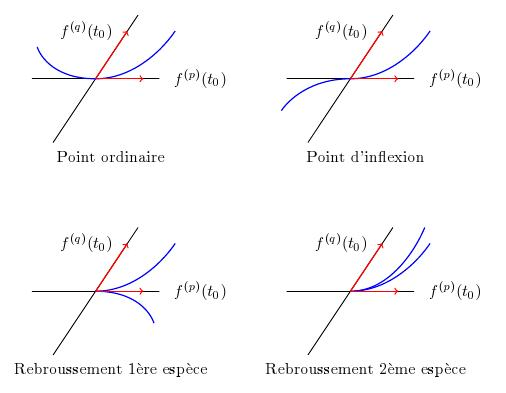
\includegraphics[height=22.em]{images/courbes.jpg}
\end{figure}


\subsubsection{Etude globale d'une courbe plane }

$E = \R^2$, $\fonction f I {\R^2} t {\begin{pmatrix} x(t) \\ y(t) \end{pmatrix}}$ $f$ de classe $\mathscr C^k, \, k \geqslant 1$.

On trace le tableau 

$$\begin{array}{c|c}
    t & \cdots \\
    \hline
    x'(t) & \cdots \\
    \hline
    y'(t) & \cdots \\
    \hline
    y(t) & \cdots \\    
\end{array}$$


\section{Intégration sur un segment }
\subsection{Théorème définition }

\begin{theoreme}{intégrale de $f \in \mathscr C^{pm}$ à valeurs dans un evn de dim finie}{}
    Soit $f : [a, b] \to E$ et $B = (e_1, \ldots, e_n)$ une base de $E$.

    Notons $\displaystyle \forall t \in [a, b], \, f(t) = \sum_{i=1}^n f_i(t)e_i$.

    On suppose que $\forall i \in \ninter{1}{n}$, $f_i$ est continue par morceaux sur $[a, b]$.

    Cela permet de définir pour $i \in \ninter{1}{n} $, $\displaystyle \int_a^b f_i(t) dt \in \K$.

    Alors si $B' = (e'_1, \ldots, e'_n)$ est une autre base de $E$, et si 
    $\displaystyle \forall t \in [a, b]$,  
    
    $\displaystyle f(t) = \sum_{i=1}^n g_i(t)e'_i$ avec 
    $g_i$ également continues par morceaux, on a :
    $$\sum_{i=1}^n \left( \int_a^b f_i(t) dt \right) e_i = \sum_{i=1}^n \left( \int_a^b g_i(t) dt \right) e'_i$$

    Ce vecteur est noté $\displaystyle \int_a^b f(t) dt$.

    On dit que $f$ est cpm sur $[a, b]$. Cette notion ne dépend donc pas 
    du choix de la base.
\end{theoreme}

\idee{"Tout bête" (Quibel)

Sinon exprimer une base dans l'autre.}

\begin{proof}
    Soit $i \in \ninter 1 n$. 

    Décomposons $e_i = \displaystyle \sum_{j=1}^n a_{i,j} e'_j$.

    On a donc $\forall t \in [a, b]$, 

    \begin{align*}
        f(t) & = \sum_{i=1}^n f_i(t) \sum_{j=1}^n a_{i,j} e'_j \\
        & = \sum_{j=1}^n \left( \sum_{i=1}^n a_{i,j} f_i(t) \right) e'_j
    \end{align*}

    Par unicité des coordonnée $\displaystyle g_j(t) = \sum_{i=1}^n a_{i,j} f_i(t)$.

    Donc $g_j$ est continue par morceaux et 

    \begin{align*}
        \sum_{i=1}^n \left( \int_a^b g_i(t) dt \right) e'_i & = \sum_{j=1}^n \left( \int_a^b \sum_{i=1}^n a_{i,j} f_i(t) dt \right) e'_j \\
            & = \sum_{j=1}^n \int_a^b \sum_{i=1}^n a_{i,j} f_i(t) dt e'_j \\
            & = \sum_{j=1}^n \sum_{i=1}^n a_{i,j} \left( \int_a^b f_i(t) dt \right) e'_j \\
            & = \sum_{i=1}^n \left( \int_a^b f_i(t) dt \right) \underbrace{\sum_{j=1}^n a_{i,j} e'_j}_{e_i} \\ 
    \end{align*}
\end{proof}

\subsubsection{Notation }

Soit $f$ continue par morceaux sur $[a, b]$. Alors on note indifféremment
$$\int_a^b f(t) dt = \int_a^b f = \int_{[a, b]} f \in E$$

\subsection{Propriétés }


\begin{proposition}{linéarité de l'intégrale }{}
    L'ensemble $\mathscr C^{pm}([a, b], E)$ est un $\K$-espace vectoriel et 
    $$ \fonction{}{\mathscr C^{pm}([a, b], E)}{E}{f}{\int_a^b f(t) dt}$$ 
    est linéaire. 
\end{proposition}

% \idee{Coordonnée par coordonnée.}

\begin{proof}
    Soit $B = (e_1, \ldots, e_n)$ une base de $E$, et notons 
    
    $\displaystyle \forall t \in [a, b], \, f(t) = \sum_{i=1}^n f_i(t)e_i$ et
    $\displaystyle g(t) = \sum_{i=1}^n g_i(t)e_i$ alors 

    $\displaystyle \forall t \in [a, b], \, (\alpha f + \beta g)(t) = \sum_{i=1}^n (\alpha f_i(t) + \beta g_i(t))e_i$.

    Donc $\alpha f + \beta g$ est cpm et par def,

    \begin{align*}
        \int_a^b (\alpha f + \beta g)(t) dt & = \sum_{i=1}^n \left( \int_a^b (\alpha f_i(t) + \beta g_i(t)) dt \right) e_i\\
        & = \sum_{i=1}^n \left( \alpha \int_a^b f_i(t) dt + \beta \int_a^b g_i(t) dt \right) e_i\\
        & = \alpha \sum_{i=1}^n \left( \int_a^b f_i(t) dt \right) e_i + \beta \sum_{i=1}^n \left( \int_a^b g_i(t) dt \right) e_i\\
        & = \alpha \int_a^b f(t) dt + \beta \int_a^b g(t) dt
    \end{align*}
\end{proof}


\begin{proposition}{Notations intégrale}{}
    Soit $f : i \to E$ cpm sur tout segment de $I$. Soient $a, b \in I$.

    Si $a < b$, alors $\displaystyle \int_a^b f(t) dt = \int_{[a, b]} f$

    Si $a = b$, par convention $\displaystyle \int_a^b f(t) dt = 0_E$

    Si $a > b$, alors $\displaystyle \int_a^b f(t) dt = - \int_{[b, a]} f$
    
\end{proposition}


\begin{proposition}{relation de Chasles}{}
    Soit $f : I \to E$ cpm sur tout segment de $I$. Soient $a, b, c \in I$.

    Alors $\displaystyle \int_a^c f(t) dt = \int_a^b f(t) dt + \int_b^c f(t) dt$.
    
\end{proposition}

\begin{proof}
    Coordonnée par coordonnée.
\end{proof}

\begin{theoreme}{composition intégrale par une application linéaire}{}
    Soit $f \in \mathscr C^{pm}([a, b], E)$, et soit $F$ un $\K$-evn de dim finie, et 
    $L \in \mathscr L(E, F)$.

    Alors $L \circ f \in \mathscr C^{pm}([a, b], F)$ et $\displaystyle \int_a^b L(f(t)) dt = L\left( \int_a^b f(t) dt \right)$.
\end{theoreme}

\idee{Coordonnée par coordonnée, as usual.}

\begin{proof}
    Soit $(e_1, \ldots, e_n)$ une base de $E$, et $(b_1, \ldots, b_q)$ une base de $F$.

    Posons $\displaystyle \forall t \in [a, b], \, f(t) = \sum_{i=1}^n f_i(t)e_i$.

    Donc $\displaystyle (L \circ f)(t) = \sum_{i=1}^n f_i(t)L(e_i)$.

    Décomposons pour tout $i$, $\displaystyle L(e_i) = \sum_{j=1}^q a_{j, i} b_j$.

    \begin{align*}
        (L \circ f) (t) & = \sum_{i=1}^n f_i(t) \sum_{j=1}^q a_{j, i} b_j \\
        & = \sum_{j=1}^q \underbrace{\left( \sum_{i=1}^n a_{j, i} f_i(t) \right)}_{g_j(t)} b_j
    \end{align*}

    Les $f_i$ sont cpm donc $g_k$ aussi, donc $L \circ f$ est cpm et par def : 

    \begin{align*}
        \int_a^b L \circ f & = \sum_{j=1}^q \left( \int_a^b g_j(t) dt \right) b_j \\
        & = \sum_{j=1}^q \left( \int_a^b \sum_{i=1}^n a_{j, i} f_i(t) dt \right) b_j \\
        & = \sum_{i = 1}^n \sum_{k = 1 }^{q } \int_{a }^{b } a_{k, i} f_i(t) dt b_k \\
        & = \sum_{i=1}^n \left( \int_a^b f_i(t) dt \right) \sum_{k=1}^q a_{k, i} b_k \\
        & = L \left( \sum_{i = 1 }^{n } \int_{a }^{b } f_i(t) \text d t e_i \right) \\
        & = L \left( \int_a^b f(t) dt \right)
    \end{align*}
\end{proof}

\subsection{Sommes de Riemann}

\begin{definition}{somme de Riemann}{}
    Soit $N \geqslant 2$ et $f \in \mathscr C^{pm}([a, b], E)$.

    On appelle somme de Riemann à gauche (resp. à droite) pour $f$ sur $[a, b]$ associée à la 
    subdivision régulière en $N$ segments le vecteur 
    $$R_{g, N, f, [a, b]} = \frac{b-a} N \sum_{k=0}^{N-1} f\left( a + k \frac{b-a}{N} \right)$$

    Resp. $\displaystyle R_{d, N, f, [a, b]} = \frac{b-a} N \sum_{k=1}^{N} f\left( a + k \frac{b-a}{N} \right)$
\end{definition}

\begin{remarque}
    La notation des R avec 50 indices est pas universelle
\end{remarque}

\begin{proposition}{}{}
    Soit $f \in \mathscr C^{pm}([a, b], E)$. Alors les sommes de Riemann pour $f$ convergent vers 
    $\displaystyle \int_a^b f(t) dt$ quand $N \to +\infty$.

    On a donc 
    $$ \frac{b - a }{N } \sum_{k = 0 }^{N - 1 } f\left( a + k \frac{b - a } N \right) \limit{N}{+ \infty} \int_a^b f(t) dt$$
    $$ \frac{b - a }{N } \sum_{k = 1 }^{N} f\left( a + k \frac{b - a } N \right) \limit{N}{+ \infty} \int_a^b f(t) dt$$

\end{proposition}

\idee{Surprise surprise, coordonnée par coordonnée.}

\begin{proof}
    \begin{align*}
        R_{g, N, f, [a, b]} & = \frac{b - a }{N } \sum_{k = 0 }^{N - 1 } \sum_{i = 1 }^{n } f_i\left( a + k \frac{b - a } N \right) e_i \\
        & = \sum_{i = 1 }^{n } \left( \frac{b - a }{N } \sum_{k = 0 }^{N - 1 } f_i\left( a + k \frac{b - a } N \right) \right) e_i \\
        & \limit{N}{+ \infty} \sum_{i = 1 }^{n } \left( \int_a^b f_i(t) dt \right) e_i \\
        & = \int_a^b f(t) dt
    \end{align*}
\end{proof}

\begin{theoreme}{inégalité triangulaire pour l'intégrale}{}
    Munisson $E$ d'une norme $||\cdot||$. Soit $f \in \mathscr C^{pm}([a, b], E)$.
    
    Alors $||f|| \in \mathscr C^{pm}([a, b], \R)$ et
    $$\left|\left| \int_a^b f(t) dt \right|\right| \leqslant \int_a^b ||f(t)|| dt$$
\end{theoreme}

\idee{Sommes de Riemann + passage à la limite.}

\begin{proof}
    $||f||$ est cpm par compo car $||\cdot||$ est continue.

    Soit $N \geqslant 1$, alors 

    \begin{align*}
        \left|\left| R_{g, N, f, [a, b]} \right|\right| & = \left|\left| \frac{b-a}{N} \sum_{k=0}^{N-1} f\left( a + k \frac{b-a}{N} \right) \right|\right| \\
        & \leqslant \frac{b-a}{N} \sum_{k=0}^{N-1} \left|\left| f\left( a + k \frac{b-a}{N} \right) \right|\right| \\
        & \leqslant R_{g, N, ||f||, [a, b]}
    \end{align*}

    Et donc par passage à la limite, 
    $$\left|\left| \int_a^b f(t) dt \right|\right| \leqslant \int_a^b ||f(t)|| dt$$
\end{proof}


\subsection{Intégrale de la borne supérieure }

\begin{theoreme}{Primitive fonction vectorielle}{}
    Soit $f \in \mathscr C(I, E)$ et $a \in I$. 

    Alors $\fonction{F}{I}{E}{x}{\int_a^x f(t) dt}$ est de classe $\mathscr C^1$ sur $I$ et 
    vérifie $F' = f$.

    $F$ est appelée la primitive de $f $ qui s'annule en $a$. 
\end{theoreme}

\idee{Coordonnée par coordonnée.}

\begin{proof}
    Notons $B = (e_1, \ldots, e_n)$ une base de $E$, et $\forall t \in I, \, f(t) \displaystyle = \sum_{i = 0 }^{ n } f_i(t) e_i$

    Donc $\displaystyle F(x) = \sum_{i = 0 }^{ n } \left( \int_a^x f_i(t) dt \right) e_i$.

    Par le théorème fondamental pour les fonctions réelles, $F_i$ est de classe $\mathscr C^1$ et $F_i' = f_i$.
\end{proof}

\begin{corollaire}{calcul d'intégrale}{}
    Soit $f \in \mathscr C(I, E)$ et $F \in \mathscr C^1(I, E)$ tel que 
    $F' = f$, alors $F$ est appelée une primitive de $f$. Alors $\forall a, b \in I$, 
    
    $$\displaystyle \int_a^b f(t) dt = F(b) - F(a)$$
\end{corollaire}

\idee{Prendre deux primitives différentes. }

\begin{proof}
    Posons $\forall x \in I, \, G(x) = \int_a^x f(t) dt$.

    Par le théorème, $G' = f = F'$ donc $(F - G)' = 0$ et donc $F - G$ est constante, 
    donc $F(b) - F(a) = G(b) - G(a) = \int_a^b f(t) dt$.
\end{proof}


\subsubsection{Recherche de primitives }

$$\renewcommand{\arraystretch}{1.6}
\begin{array}{|c|c|c|}
    \hline
    I & f(x) & \int_{a }^{x } f(t) dt \\
    \hline
    \R & x^n & \frac{x^{n+1}}{n + 1} \\
    \hline
    \R^*_+ & x^\alpha, \alpha \neq -1 & \frac{x^{\alpha + 1}}{\alpha + 1} \\
    \hline
    \R^*_+ \text{ ou } \R_-^*& \frac 1 x & \ln |x| \\
    \hline
    \R & e^x & e^x \\
    \hline
    \R & \cos x & \sin x \\
    \hline
    \R & \sin x & -\cos x \\
    \hline
    \R & \cosh x & \sinh x \\
    \hline
    \R & \sinh x & \cosh x \\
    \hline
    \R & \frac 1 {1 + x^2} & \arctan x \\
    \hline
    ]-1, 1[ & \frac 1 {\sqrt{1 - x^2}} & \arcsin x\\
    \hline
\end{array}$$

\subsubsection{Intégration par parties }

Soient $u, v \in \mathscr C^1([a, b], \K)$.

Alors $$\int_{a }^{b } u'\cdot v = \left[ u \cdot v \right]_{a }^{b } - \int_{a }^{b } u \cdot v'$$

\subsubsection{Changement de variable }

Soit $\varphi \in \mathscr C^1(J, I)$ et $\alpha, \beta \in J$, 
$\varphi(\alpha) = a, \, \varphi(\beta) = b$.

Soit $f \in \mathscr C(I, E)$. Alors $$\int_\alpha^\beta f(\varphi(u)) \varphi'(u) du = \int_a^b f(t) dt$$
En posant $t = \varphi(u)$, donc $dx = \varphi'(u) du$.

Changements de variable usuels : 

$$\renewcommand{\arraystretch}{2.1}
{\everymath{\displaystyle}
\begin{array}{|c|c|}
    \hline 
    \text{\textbf{Intégrale}} & \text{\textbf{changement}} \\
    \hline
    \displaystyle \int_a^b f(t^2)t dt & x = t^2 \; dx = 2t dt \\
    \hline
    \int_a^b f(\cos t) \sin t dt & x = \cos t \; dx = -\sin t dt \\
    \hline
    \int_a^b F(e^t) dt & \substack{x = e^t \; dx = e^t dt \\ t = \ln(x) \; dt = \frac{dx} x} \\
    \hline 
    \int_{a }^{b } F(\cos t, \sin t) dt, \; F \in \K(X) & \substack{u = \tan \frac t 2, \; t = 2 \arctan u \; dt = \frac{2 du}{1 + u^2} \\ \cos t = \frac{1 - u^2}{1 + u^2} \; \sin t = \frac{2u}{1 + u^2}} \\
    \hline
    \int_{a }^{b } F(x, \sqrt{1 - x^2}) dx & x = \sin t \\
    \hline
    \int_{a }^{b } F(x, \sqrt{x^2 - 1}) dx & x = \cosh t \\
    \hline
    \int_{a }^{b } F(x, \sqrt{1 + x^2}) dx & x = \sinh t \\
    \hline
\end{array}}$$

\subsubsection{Décomposition en éléments simples }

\begin{exemple}
    $\displaystyle I = \int_0^x \sqrt{\tan t} \text d t$, $x \in [0, \frac \pi 2[$.

    Posons $u = \sqrt{\tan t}$, donc $t = \arctan(u^2)$, $dt = \frac{2u}{1 + u^4} du$.

    Donc $\displaystyle I = \int_0^{\sqrt{\tan x}} \frac{2u^2}{1 + u^4} du$.

    Décomposition en éléments simples : $\frac{2X^2}{X^4 + 1}$

    $1 + X^4 = (1 + X^2)^2 -2X^2 = (1 - \sqrt 2 X + X^2)(1 + \sqrt 2 X + X^2)$

    Donc $\displaystyle \frac{2X^2}{1 + X^4} = \frac{aX + b}{X^2 - \sqrt 2 X + 1} + \frac{cX + d}{X^2 + \sqrt 2 X + 1}$.

    En évaluant en 0 : $b + d = 0$.

    Limite en $+\infty : 0 = a + c$. 

    On a donc : $\displaystyle \frac{2X^2}{1 + X^4} = \frac{aX + b}{X^2 - \sqrt 2 X + 1} - \frac{aX + b}{X^2 + \sqrt 2 X + 1} = \frac{(aX + b)(2 \sqrt 2 X)}{X^4 + 1}$.

    Donc $b = 0$ et $a = \frac{\sqrt 2 }{2}$. Donc $\forall u, $

    \begin{align*}
        \frac{2 u^2}{1 + u^4} & = \frac 1 2 \left[\frac{\sqrt 2 u }{u^2 - \sqrt 2 u + 1} - \frac{\sqrt 2 u }{u^2 + \sqrt 2 u + 1}\right]\\
        & = \frac 1 2 \left[ \frac 1 {\sqrt 2} \frac{2u - \sqrt 2}{u^2 - \sqrt 2 u + 1} + \frac 1 {u^2 - \sqrt 2 u + 1} - \frac 1 {\sqrt 2} \frac{2u + \sqrt 2}{u^2 + \sqrt 2 u + 1} + \frac 1 {u^2 + \sqrt 2 u + 1} \right]\\
        & = \frac 1 {2 \sqrt 2} \left[ \frac{2u - \sqrt 2}{u^2 - \sqrt 2 u + 1} - \frac{2u + \sqrt 2}{u^2 + \sqrt 2 u + 1} \right] + \frac 1 2 \left[ \frac{1}{\left( u - \frac{\sqrt 2 }{2} \right)^2 + \frac 1 2} + \frac{1}{\left( u + \frac{\sqrt 2}{2} \right)^2 + \frac 1 2} \right]\\
        & = \frac 1 {2 \sqrt 2} \left[ \frac{2u - \sqrt 2}{u^2 - \sqrt 2 u + 1} + \frac 1 {(\sqrt 2 u - 1)^2 + 1} + \frac 1 {(\sqrt 2 u + 1)^2 + 1} \right]
    \end{align*}

    Donc $\displaystyle I = \left[ \frac{1 }{2 \sqrt 2 } \ln(u^2 - \sqrt 2 u + 1) - \ln(u^2 + \sqrt 2 u + 1) + \frac{\arctan(\sqrt 2 u - 1)}{\sqrt 2} + \frac{\arctan(\sqrt 2 u + 1)}{\sqrt 2} \right]_0^{\sqrt{\tan x}}$
\end{exemple}

\begin{theoreme}{Inégalité des accroissements finis}{}
    Soit $f \in \mathscr C^1(I, E)$. On suppose $\exists M > 0, \, \forall x \in I, \, ||f'(x)|| \leqslant M$.

    Alors $\forall a, b \in I$, 

    $$||f(b) - f(a)|| \leqslant M |b - a|$$
\end{theoreme}

\idee{Inégalité triangulaire des intégrales }

\begin{proof}

    $f(b) - f(a) = \int_a^b f'(t) dt$.

    Donc $\displaystyle ||f(b) - f(a)|| \leqslant \int_a^b ||f'(t)|| dt \leqslant \int_a^b M dt = M |b - a|$.
\end{proof}


\subsection{Formule de Taylor }

\begin{proposition}{Formule de Taylor avec reste intégral}{}
    Soit $f \in \mathscr C^{n + 1}(I, E)$, $a, b \in I$. 

    $$f(b) = \sum_{k = 0 }^{n } \frac{(b - a)^k}{k!} f^{(k)}(a) + \int_a^b \frac{f^{(n + 1)}(t)}{n!} (b - t)^n dt$$
\end{proposition}

\begin{proof}
    Composante par composante.
\end{proof}

\begin{proposition}{Inégalité de Taylor-Lagrange}{}
    Soit $f \in \mathscr C^{n + 1}(I, E)$, $a, b \in I$. On suppose $\exists M > 0, \, \forall t \in [a, b], \, ||f^{(n + 1)}(t)|| \leqslant M$.

    Alors $$\left|\left| f(b) - \sum_{k = 0 }^{n } \frac{(b - a)^k}{k!} f^{(k)}(a) \right|\right| \leqslant \frac{M |b - a|^{n + 1}}{(n + 1)!}$$
\end{proposition}

\begin{proof}
    On prend $a < b$

    \begin{align*}
    \left|\left| f(b) - \sum_{k = 0}^n \frac{(b - a)^k}{k!} f^{(k)}(a) \right|\right|  & = \left|\left| \int_a^b \frac{f^{(n + 1)}(t)}{n!} (b - t)^n dt \right|\right| \\
     & \leqslant \int_a^b \left| \frac{(b - t)^n}{n!} \right| M dt \\
        & \leqslant M \int_{a }^{b } \frac{(b - t)^n}{n!} dt \\
        & = M \frac{(b - a )^{n + 1}}{(n+ 1)!}
    \end{align*}
\end{proof}

\begin{proposition}{Formule de Taylor-Young}{}
    Soit $f \in \mathscr C^n(I, E)$, alors pour $a \in I$, $h \in \R$ tel que $a + h \in I$, on a

    $$f(a + h) = \sum_{k = 0 }^{n } \frac{h^k}{k!} f^{(k)}(a) + o(h^n)$$
\end{proposition}

\begin{proof}
    Composante par composante.
\end{proof}




